% Chapter 1

\chapter{Introducción}
% Write in your own chapter title
\label{Capitulo 1}
\lhead{Capítulo 1. \emph{Introducción}} % Write in your own chapter title to set the page header

%-->
% dispositivos móviles con sensores\\
% aplicaciones\\
% browser\\
% aplicaciones web\\
% frameworks\\
% MVC\\
% Continuations\\
% Sensibilidad al contexto\\
%- Estado del arte (continuations y sensibilidad al contexto)\\
%- Motivación\\
%- Contribuciones\\
%- Esquema\\
%-->

%Existe una gran variedad de dispositivos móviles, ya sean de carácter específico o de propósito general, que cuentan con funcionalidades cada vez más novedosas.

%En la actualidad, los dispositivos móviles son enriquecidos con sensores encargados de medir ciertos valores del medio ambiente (como el micrófono, el sensor táctil, el \emph{GPS}\footnote{Del inglés ``Global Positioning System''.}, el acelerómetro, la cámara, el sensor de luminosidad, el giróscopo, etc.), y actuadores encargados de modificarlo (como la pantalla, el parlante, el motor vibrador, etc.).

%Cada dispositivo posee su propia configuración de \emph{hardware} (compuesta por sensores y actuadores, capacidad de procesamiento, capacidad de almacenamiento, y otros) y de \emph{software} (un Sistema Operativo, de aquí en adelante OS\footnote{Del inglés ``Operating System''.}). Éstas configuraciones permiten ciertas flexibilidades e imponen ciertas restricciones en el desarrollo de aplicaciones.

%Éstas aplicaciones dependientes de la \emph{configuración} son denominadas \emph{aplicaciones nativas}. Como consecuencia, una aplicación puede verse representada por varias aplicaciones nativas, una para cada configuración.

%En caso de ser necesario, una aplicación nativa debe ser desarrollada nuevamente para que la aplicación pueda ejecutarse en una configuración no soportada. Por ejemplo, una aplicación nativa desarrollada para el OS \emph{iOS}\footnote{OS del iPhone.} debe ser portada (o desarrollada nuevamente) para que pueda funcionar en un dispositivo móvil con \emph{Android}\footnote{OS disponible en una gran variedad de dispositivos.}.

%Un caso particular de aplicación nativa son los \emph{web browsers}, los cuales permiten recuperar, presentar y atravesar los recursos disponibles en la \emph{World Wide Web (más conocida como WWW)}. Entre los recursos disponibles se encuentran las imágenes, los videos, las páginas web, los fragmentos de programas o inclusive aplicaciones completas, entre otros.

%A este último tipo de aplicaciones que son accedidas y ejecutadas mediante la utilización de un web browser se las denomina \emph{aplicaciones web}.

%- En los últimos años se viene incrementado la cantidad de sensores existentes en los diferentes dispositivos tecnológicos. Cada ves más díscos rígidos, procesadores, electrodomésticos y dispositivos móviles (desde teléfonos ``inteligentes'' hasta autos) cuentan con la posibilidad de realizar acciones mas precisas teniendo en cuenta la información brindada por estos sensores.

Hace ya algún tiempo que las \emph{páginas web} han evolucionado a lo que hoy se denomina \emph{aplicaciones web}. Estas aplicaciones, que son accedidas y ejecutadas mediante la utilización de un \emph{navegador web}, suelen modificar su contenido a partir de la interacción con el usuario.

El desarrollo de estas aplicaciones, a diferencia de una página web convencional, suele ser realizado mediante la utilización de algún framework\footnote{Abstracción que reúne cierto código fuente genérico, permitiendo la reutilización mediante la especialización de cierta funcionalidad.} que simplifique la comunicación entre un \emph{modelo de negocio} y cada uno de los posibles \emph{usuarios}.

Existen varios frameworks que permiten simplificar las tareas de creación, actualización y mantenimiento de las aplicaciones web. La mayoría consisten en una implementación del esquema \emph{Model-View-Controller\cite{Krasner88,Gamma95} (en adelante MVC)}, aunque también existe una minoría que plantea la utilización del concepto de \emph{continuations}.

Los frameworks que implementan el esquema \emph{MVC} contienen 3 tipos de objetos que pueden ser especializados: el \emph{Modelo}, se encarga de la lógica de negocios; la \emph{Vista}, se encarga de la salida del sistema; y el \emph{Controlador}, se encarga de la entrada al sistema. Este tipo de framework suele cumplir con una arquitectura de \emph{Transferencia del Estado Representacional\footnote{Del inglés ``REpresentational State Transfer''.} (en adelante abreviado como REST)} que garantiza que por cada interacción del usuario con el modelo de negocios, el controlador y la vista no mantendrán información de las transacciones e interacciones que realiza el usuario.

Por otra parte, existe una minoría de las aplicaciones web que son realizadas a partir del concepto de \emph{continuations}. Estas conservan en el servidor el estado del cliente a partir de la utilización de un \emph{Componente} como átomo de construcción. Éste cumple las mismas funciones que una Vista y un Controlador, primero evalúa la solicitud realizada por el cliente para poder realizar los cambios adecuados en el modelo, y luego genera el resultado que será presentado como respuesta en el navegador web.

Una \emph{aplicación web} según el concepto de continuations, es un componente compuesto por múltiples subcomponentes (ya sean estos simples o nuevamente compuestos por otros). Además cada uno establece su flujo de trabajo, permitiendo establecer ciclos y comprobaciones mediante la utilización del lenguaje con el cual se encuentre programado el framework.

Estos frameworks que facilitan el desarrollo de las interfaces gráficas que luego serán utilizadas por los usuarios, por lo general no utilizan una parte de la información disponible en un dispositivo tecnológico (como el estado de sus sensores). De esta forma, las aplicaciones web carecen de la posibilidad de mejorar aún mas la interacción con el usuario.

En varios documentos científicos\cite{Challiol06,Fortier07,Challiol08,Kapitsaki09,Fortier09} se proponen alternativas para incorporar la utilización de sensores a frameworks que implementan el esquema MVC. Como contraparte, hasta el momento, no he encontrado una alternativa para realizar lo mismo con una aplicación web desarrollada con \emph{continuations}.


\section{Estado del arte}

% Dado que esta tesis pretende obtener un resultado a partir de la combinación de dos líneas de investigación: por un lado el concepto de \emph{continuations} y por el otro la \emph{sensibilidad del contexto}; se prosigue con el desarrollo cronológico de cada una de ellas.

Dado que esta tesis pretende obtener un resultado a partir de la combinación de dos líneas de investigación: por un lado aplicaciones web que utilizan el concepto de \emph{continuations} y por el otro la utilización de sensores como medio de interacción con el usuario (lo cual suele ser visto como un aspecto de la  \emph{sensibilidad del contexto}\cite{Schilit94}); se prosigue con el desarrollo cronológico de cada una de ellas\footnote{La palabra Contexto es utilizada en ambas áreas, en tanto se utilizará la frase \emph{contexto de ejecución} para referirse al contexto del área relacionada con continuations. Se reservará la palabra \emph{contexto} para lo relacionado con la sensibilidad al contexto.}.


\subsection{Continuations}

Según la investigación histórica del surgimiento del concepto de \emph{continuations} realizada por \emph{Reynolds}, ``Adriaan van Wijngaarden fue el primero en describir una técnica semejante a \emph{continuations} en el año 1964, en la \emph{IFIP Working Conference of Formal Language Description Languages}''\cite[p.~234]{Reynolds93}.

De acuerdo a lo que \emph{van Wijngaarden} describe:

\begin{quote}
Al proveer a cada declaración de procedimiento con un parámetro formal extra - especificado como \textbf{etiqueta} - e insertar al final del cuerpo una sentencia \textbf{goto} llamando al parámetro formal. Consecuentemente, se llamará al proce\-dimiento estableciendo una etiqueta en la posición del parámetro extra correspondiente.\cite[p.~14]{vanWijngaarden66}
\end{quote}

De esta manera \emph{van Wijngaarden}, es el primero en intentar una abstracción\footnote{Realizada en el lenguaje Algol60} (que evita la utilización directa de \emph{goto} y \emph{labels}) para delegar el control de la pila de ejecución en el procedimiento al que está llamando.

Según \emph{Reynolds}, esta abstracción fue influyendo en otros autores y evolucionando, hasta que entre 1969 y 1970 Christopher Wadsworth nombró a esta abstracción \emph{continuations}. Actualmente, el nombre formal es \emph{Continuation-passing style} (también abreviado como CPS).

Desde este momento en adelante es importante destacar que las implementaciones de continuations no almacenan datos del programa, sólo almacenan el \emph{contexto de ejecución}.

En 1988, \emph{Rees et al.} transforman a \emph{Scheme} en el primer lenguaje en soportar de forma nativa la abstracción de continuations, denominándose a este tipo de implementaciones \emph{first-class continuations}\cite[p.~3]{Rees88}.

Recién en 2003, \emph{Queinnec} sugiere la utilización de continuations en aplicaciones web como alternativa a un esquema orientado a páginas\cite{Queinnec01}. Para esto plantea el siguiente caso:

\begin{quote}
Los navegadores brindan la funcionalidad para `retroceder' y `clonar'. Los clientes (por ejemplo, usuarios de los navegadores web) pueden utilizar éstas facilidades para descubrir el comportamiento del sitio con la actitud de `¿qué pasa si?'. Desde un formulario, el cliente envía información al servidor, examina el resultado (posiblemente con algo de interacción) y vuelve al formulario original si el resultado no luce prometedor. En lugar de volver atrás al formulario original, el cliente podría clonar el formulario original o \emph{agendarlo}\footnote{En inglés ``bookmark it''.}. En todos los casos, el cliente tiene la oportunidad de volver a responder a un formulario. ¡Aún más, clonarlos permite que el cliente envíe, de forma concurrente, nuevas respuestas para formularios ya respondidos!.\cite[p.~2]{Queinnec01}
\end{quote}

\emph{Queinnec}, además presenta una variante que permite anular desde el servidor el proceso de `retroceder', devolviendo al cliente el formulario correspondiente, de acuerdo con lo que el modelo de negocios establezca. Y cancelando cualquier posibilidad de volver a cargar un `formulario' ya completo.

Esto proporciona una forma de solucionar ciertos inconvenientes (relacionados con la manipulación de transacciones) aún no resueltos de forma genérica con el esquema MVC.

En la actualidad, utilizando las nociones presentadas por \emph{Quiennec}, Seaside es el framework mas usado por los desarrolladores dentro del conjunto de las aplicaciones web basadas en continuations. Esto le ha permitido, a su vez, liderar en el área de la investigación con el fin de brindar soportar a las nuevas tecnologías que continúan surgiendo.


\subsection{Sensibilidad al contexto}

La otra linea de investigación fundamental para el desarrollo de esta tesis es la sensibilidad al contexto.

La \emph{computación sensible al contexto} es definida por \emph{Schilit y Theimer} en 1994, al afirmar que ``se produce cuando un \emph{software} tiene la habilidad de descubrir y reaccionar ante cambios en el entorno en el que se encuentra un usuario móvil''\cite[p.~23]{Schilit94}. Además agregaron que un entorno puede estar compuesto por dispositivos, personas y servicios.

Según \emph{Dey}, \emph{Schilit  y Theimer} realizaron una definición muy acotada de contexto que sólo contempló a la localización y proximidad; por lo que en el 2001, sugiere una definición más amplia de contexto afirmando:

\begin{quote}
Contexto es cualquier información que pueda ser usada para caracterizar la situación de una entidad. Una entidad es una persona, un lugar, o un objeto que es considerado relevante para la interacción entre un usuario y una aplicación; incluyendo al mismo usuario y/o la misma aplicación dentro de los objetos posibles.\cite[p.~3]{Dey01}
\end{quote}

Como consecuencia de la definición demasiado inclusiva de \emph{Dey}, \emph{Efstratiou} en el 2004 propone una subclasificación describiendo:

\begin{quote}
Las aplicaciones adaptativas sensibles al contexto, son las que modifican su comportamiento (se adaptan) de acuerdo a los cambios en el contexto de la aplicación. El término contexto es usado de acuerdo con \emph{la definición de Dey} siendo cualquier información que pueda ser usada para caracterizar la situación de una entidad.\cite[p.~4]{Efstratiou04}
\end{quote}

De esta forma, \emph{Efstratiou} propone que las \emph{aplicaciones adaptativas sensibles al contexto} son un subconjunto de las \emph{aplicaciones sensibles al contexto} y un superconjunto que contiene a las \emph{aplicaciones adaptativas tradicionales} (ver Figura \ref{AdaptiveContextAwareSystems}).

\begin{figure}[ht!]
\centering
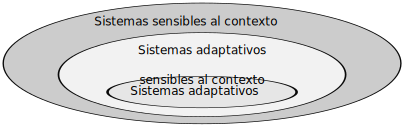
\includegraphics[scale=1]{ContextAwareSystems}
\caption{Sistemas adaptativos sensibles al contexto}
\label{AdaptiveContextAwareSystems}
\end{figure}

\emph{Efstratiou}, continúa detallando que ``se espera que una aplicación adaptativa sensible al contexto, sea capaz de reaccionar a una variedad de \emph{disparadores contextuales}\footnote{Del inglés ``Contextual triggers''.}''. Además, plantea que ``la interacción de múltiples aplicaciones sensibles al contexto que se adaptan a distintos disparadores de entornos, al interrelacionarse podrían causar inestabilidades y comportamientos no deseados''.

Por último, en su tesis explica como coordinar las diferentes aplicaciones, y como resolver los conflictos entre los distintos intereses que puede disparar cada aplicación. Además plantea como involucrar las preferencias del usuario y promover la extensibilidad.

Por otra parte, en 2008, \emph{Costanza} plantea una postura levemente diferente a la de \emph{Dey}. \emph{Costanza} justifica que ``\emph{la definición de Dey} distingue entre información relevante y no relevante, lo cual es importante cuando se está modelando sistemas de adquisición y razonamiento de contextos'', mientras que su definición ``apunta a formas estructuradas de ver cómo se ve afectado el comportamiento del programa en función del contexto, lo cual debería ser abordado por construcciones de uso general y así ser independiente de los tipos de información de contexto de los cuales depende''\cite[p.~1]{Costanza08}.

\emph{Costanza} propone un paradigma de \emph{Programación Orientada a Contextos} (en adelante COP\footnote{Del inglés ``Context-Oriented Programming''.}). En este paradigma, ``los programas se suelen dividir en \emph{variaciones} (o diferenciales) de comportamiento que pueden ser activadas y combinadas en tiempo de ejecución con alcances bien definidos''. El COP ``se centra en construcciones de programación que habilitan el agrupamiento, el referenciamiento, y la activación/desactivación de capas de variaciones en el comportamiento''. Además presenta a \emph{ContextL} que surge como extensión al \emph{Common Lisp Object System}\footnote{El cual es la extensión del lenguaje Common List que brinda soporte a la Programación Orientada a Objetos (o Object Oriented Programming).}, permitiendo asociar la definición de \emph{clases}, \emph{métodos} y \emph{funciones} a distintas \emph{capas} (o variaciones).

\emph{Chang et al.} continuando por la línea de \emph{Dey} y \emph{Efstratiou}, en el 2007, intuye que una aplicación web necesita adaptarse a sí misma a diferentes contextos de ejecución para garantizar cierta \emph{calidad de servicio} (en adelante QoS\footnote{Del inglés ``Quality Of Service''.})\cite[p.~1]{Chang07}. Específicamente, describe que una \emph{aplicación web sensible al contexto} requiere:
\begin{itemize}
	\item La habilidad de \emph{auto-adaptarse} a los entornos específicos de su implementación.
	\item El potencial de \emph{evolucionar} bajo una forma general, tanto a partir del entorno de ejecución como de la forma de uso.
\end{itemize}

Principalmente, Chang menciona que las ``aplicaciones web son esencialmente distribuidas y heterogéneas'', a partir de que existen 2 lugares en donde se puede realizar el procesamiento: el \emph{cliente} y el \emph{servidor}, y en ambos existen alternativas en cuanto a la tecnología utilizada y el entorno disponible. Como consecuencia de esto, desarrolla ``la descomposición de una aplicación web en componentes que serán utilizados si es que el contexto así lo requiere''. Además detalla que es suficiente con que una aplicación se adapte en el momento de \emph{descargarse al cliente}, descartando así la necesidad de adaptación en tiempo de ejecución.

Hacia comienzos del 2009, \emph{Kapitsaki et al.} prosigue en la investigación de sensibilidad al contexto en combinación con aplicaciones web y descarta que la adaptación al contexto deba realizarse dentro del modelo de negocios. Relacionando la sensibilidad al contexto como una característica más que puede contener un Controlador (del esquema MVC)\cite{Kapitsaki09}.

De esta forma, \emph{Kapitsaki et al.} propone una arquitectura en la que, mediante la composición de un grupo de servicios (o aplicaciones web) que no son sensibles al contexto, permite la adaptación al contexto dejando al controlador como responsable de la relación entre el modelo de negocios y el modelo contextual.

También en 2009, \emph{Fortier et al.} plantea un conjunto de micro-abstracciones, que permiten lidiar con la variabilidad de los modelos sensibles al contexto en dispositivos móviles\cite{Fortier09}.


\section{Motivación}


%Teniendo en cuenta la situación cambiante de los \emph{modelos de negocio} actuales y una aplicación web desarrollada con Continuations, en donde el modelo recibe actualizaciones para adaptarse a los nuevos requisitos del sistema y la interfaz gráfica se expande para soportar pantallas específicas para ciertas situaciones del contexto.

Teniendo en cuenta el estado del arte de las aplicaciones web desarrolladas con continuations, en donde no es posible la utilización de sensores para controlar la aplicación. Y considerando las ventajas en la interacción con el usuario que brindan aquellas aplicaciones que se adaptan al contexto.

%Y considerando que no existe una alternativa que permita a una aplicación web desarrollada con Continuations utilizar la información del contexto del cliente, dado que los modelos existentes para adaptar una aplicación web utilizan un esquema MVC\cite{Challiol06,Fortier07,Challiol08,Kapitsaki09,Fortier09}.

Se propone el desarrollo de una librería, que extienda a una implementación de Continuations, para poder utilizar en el servidor la información provista por los sensores de los distintos clientes.

%Para esto se revisará la subclasificación de \emph{Efstratiou}, y a partir de ella se realizará una implementación de \emph{triggers contextuales} que contemple la modificación del contexto de cada usuario, y realice adaptaciones necesarias.

Para esto se utilizará el concepto de \emph{triggers contextuales} mencionado por \emph{Efstratiou}, y como consecuencia se propondrá una implementación de \emph{aplicación web adaptativa al contexto}.

En la solución propuesta, es necesario contemplar los requisitos de cada linea de investigación y tratar de encontrar el mejor compromiso entre ellas.


\section{Contribuciones}

Las contribuciones que se podrán desprender de esta tesis son:
\begin{itemize}
\item Principalmente, la adaptación de una aplicación web que utiliza continuations al contexto del usuario.
\item En segundo término, un análisis de los patrones de diseño que se utilicen en la realización de la librería.
\item Por último, una comparación de la librería propuesta con las librerías existentes para el esquema MVC.
\end{itemize}

Se esperan estas tres contribuciones antes mencionadas. En primera instancia se trata de proveer una librería de sensiblidad al contexto para las aplicaciones web que utilizan continuations.

Para demostrar la utilidad y funcionalidad de la librería se presentará un caso de ejemplo que adapta la aplicación web al contexto del dispositivo.

La segunda contribución es que la librería sea modificable y extensible. Al realizar un análisis de los \emph{patrones de diseño}\cite{Gamma95} utilizados se podrá entender mejor el modelo planteado.

La última contribución se enfoca en realizar una comparación de la librería propuesta y las alternativas existentes que utilizan el esquema MVC.

El alcance de esta tesis no incluirá:
\begin{itemize}
\item discusión alguna sobre la variante \emph{evolutiva} de la sensibilidad al contexto, que utiliza el análisis de las interacciones del usuario para \emph{deducir} nuevas adaptaciones al contexto;
\item pruebas de rendimiento o performance, dado que la realización de estas desviarían el objetivo de esta tesis, que es demostrar la posibilidad de mezclar las dos lineas.
\end{itemize}


\section{Esquema}

El resto de la tesis se organiza de la siguiente manera: en el \emph{Capítulo 2} se desarrollará con profundidad el concepto de continuations en el marco de las aplicaciones web. Dentro del \emph{Capítulo 3} se introducirán los conceptos esenciales sobre aplicaciones sensibles al contexto necesarios para comprender esta tesis.

En el \emph{Capítulo 4} se describirá la solución propuesta y se analizarán los patrones de diseño utilizados.

Un ejemplo completo será presentado en el \emph{Capítulo 5}, en el cual se mostrará la flexibi\-lidad de la librería en la utilización de sensores. Mientras que el \emph{Capítulo 6} mencionará las extensiones posibles para la librería, además de los límites que ésta posee.

Por último, en las \emph{Conclusiones}, se realizará una breve comparación con otros trabajos semejantes, se mencionarán los resultados de esta tesis, y algunas líneas de investigación que se desprenden de este trabajo.